\documentclass[aspectratio=169]{beamer}

\usetheme{default}
\setbeamertemplate{navigation symbols}{}
\setbeamertemplate{enumerate item}{\color{navy}\arabic{enumi}.}
\setbeamertemplate{itemize item}{\color{black}\textbullet}
\setbeamertemplate{itemize subitem}{\color{black}\textbullet}
\usepackage{booktabs}
\usepackage{xcolor}
\usepackage{tikz}
\usetikzlibrary{shapes,arrows,positioning}
\definecolor{navy}{RGB}{0, 0, 128}
\definecolor{lightblue}{RGB}{230,240,250}
\definecolor{darkgreen}{RGB}{0,100,0}
\definecolor{lightgreen}{RGB}{230,250,230}
\newcommand{\highlight}[1]{\colorbox{lightblue}{$\displaystyle\textcolor{navy}{#1}$}}
\newcommand{\highlighttext}[1]{\colorbox{lightblue}{\textcolor{navy}{#1}}}
\newcommand{\highlightgreen}[1]{\colorbox{lightgreen}{$\displaystyle\textcolor{darkgreen}{#1}$}}
% Put this in preamble after \usetikzlibrary line
\newcommand{\func}[1]{0.5 + 1.5*sin(deg(#1*3.14159/3))}

\begin{document}

\begin{frame}

Simulation requires drawing from the error term distribution

\bigskip

\begin{itemize}
\itemsep1.5em
\item<2-> Standard normal and uniform: use built-in random number generators
\item<3-> Other distributions: various transformation methods (e.g. \texttt{-log(-log(rand()))})
\item<4-> Multivariate normals: Choleski decomposition
\item<5-> Complex densities: accept-reject, importance sampling
\end{itemize}

\end{frame}

\begin{frame}

Independent random draws can be improved upon:

\bigskip

\begin{itemize}
\itemsep1.5em
\item<2-> \textcolor{navy}{Antithetic draws}: create mirror images to induce negative correlation
\item<3-> \textcolor{navy}{Halton sequences}: systematically fill the distribution space ``evenly'' 
\item<4-> Both provide better coverage than pure random draws
\item<5-> Can substantially reduce simulation error for given $R$
\end{itemize}

\onslide<6->{
\bigskip
Practical benefit: fewer draws needed for same accuracy
}

\end{frame}



\begin{frame}
\centering
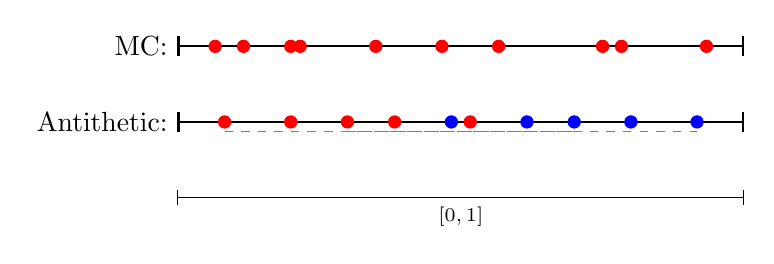
\begin{tikzpicture}[scale=1.2]
    % Pure MC
    \draw[thick, |-|] (0,0) -- (6,0);
    \foreach \x in {0.4, 0.7, 1.2, 1.3, 2.1, 2.8, 3.4, 4.5, 4.7, 5.6} {
        \fill[red] (\x,0) circle (2pt);
    }
    \node[left] at (0,0) {MC:};
    
    % Antithetic
    \draw[thick, |-|] (0,-0.8) -- (6,-0.8);
    \foreach \x in {0.5, 1.2, 1.8, 2.3, 3.1} {
        \fill[red] (\x,-0.8) circle (2pt);
        \pgfmathsetmacro{\xmirror}{6-\x}
        \fill[blue] (\xmirror,-0.8) circle (2pt);
        \draw[gray, dashed] (\x,-0.9) -- (\xmirror,-0.9);
    }
    \node[left] at (0,-0.8) {Antithetic:};
    
    \draw[|-|] (0,-1.6) -- (6,-1.6);
    \node[below, font=\scriptsize] at (3,-1.6) {$[0,1]$};
\end{tikzpicture}
\end{frame}





\begin{frame}
\centering
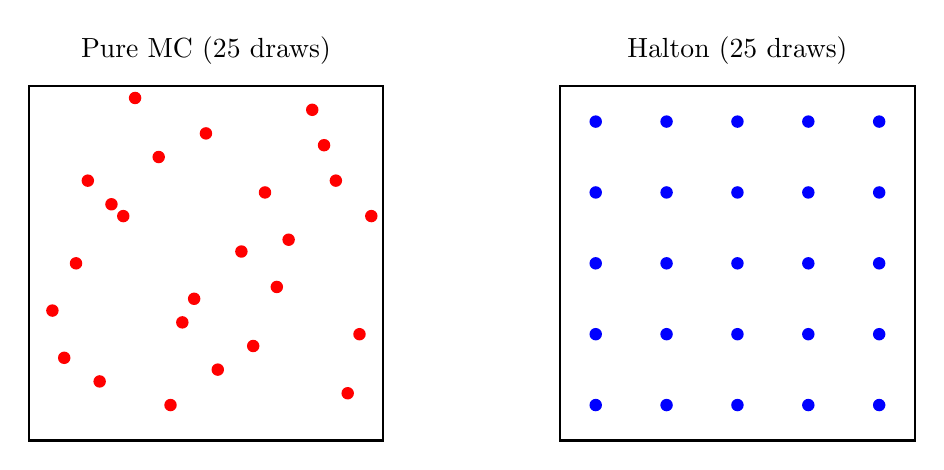
\begin{tikzpicture}[scale=1.5]
    % Pure Monte Carlo
    \begin{scope}
        \draw[thick] (0,0) rectangle (3,3);
        \node[above] at (1.5,3.1) {Pure MC (25 draws)};
        
        % Random points with seed for reproducibility concept
        \foreach \x/\y in {0.3/0.7, 2.1/1.3, 1.5/2.6, 0.8/1.9, 2.7/0.4, 
                           1.2/0.3, 2.4/2.8, 0.5/2.2, 1.8/1.6, 2.9/1.9,
                           0.2/1.1, 1.9/0.8, 0.9/2.9, 2.6/2.2, 1.4/1.2,
                           0.6/0.5, 2.2/1.7, 1.1/2.4, 2.8/0.9, 0.4/1.5,
                           1.6/0.6, 2.5/2.5, 0.7/2.0, 1.3/1.0, 2.0/2.1} {
            \fill[red] (\x,\y) circle (1.5pt);
        }
    \end{scope}
    
    % Halton Sequence
    \begin{scope}[xshift=4.5cm]
        \draw[thick] (0,0) rectangle (3,3);
        \node[above] at (1.5,3.1) {Halton (25 draws)};
        
        % Halton-like systematic pattern (base 2 and 3)
        \foreach \i in {0,...,4} {
            \foreach \j in {0,...,4} {
                \pgfmathsetmacro{\x}{0.3 + \i*0.6}
                \pgfmathsetmacro{\y}{0.3 + \j*0.6}
                \fill[blue] (\x,\y) circle (1.5pt);
            }
        }
    \end{scope}
\end{tikzpicture}
\end{frame}


\begin{frame}

When implementing simulation-based estimation:

\bigskip

\begin{itemize}
\itemsep1.5em
\item<2-> Use same draws across parameter values (prevents chatter)
\item<3-> Consider \textcolor{navy}{variance reduction techniques} for efficiency
\item<4-> Increase $R$ with sample size for SML
\item<5-> SMM offers consistency with fixed $R$ at cost of potential efficiency loss
\end{itemize}

\onslide<6->{
\bigskip
Choice depends on computational resources and model complexity
}

\end{frame}

\end{document}